\section{Weighted Model Counting with Tensor Networks}
\label{sec:algorithm}
In this section, we discuss the algorithm for literal-weighted model counting using tensor networks as outlined by \cite{DDV19}. This algorithm is presented as Algorithm \ref{alg:wmc-tn} and has three stages.

First, in the \emph{reduction} stage the input formula $\varphi$ and weight function $W$ is transformed into a tensor network $N$. We discuss in more detail in Section \ref{sec:algorithm:reduction}.

Second, in the \emph{planning} stage a plan for contracting the tensor network $N$ is determined. This plan takes the form of a \emph{contraction tree} \cite{EP14}:
\begin{definition}[Contraction Tree] \label{def:contraction-tree}
	Let $N$ be a tensor network. A \emph{contraction tree} for $N$ is a rooted binary tree $T$ whose leaves are the tensors of $N$. %, i.e. $\Lv{T} = N$.
\end{definition}
The planning stage is allowed to modify the input tensor network $N$ as long as the new tensor network $M$ contracts to an identical tensor. We discuss various heuristics for contraction trees in Section \ref{sec:algorithm:planning}.
Planning in Algorithm \ref{alg:wmc-tn} is an anytime process: we heuristically generate better contraction trees until one is ``good enough'' to use. The trade-off between planning and executing is governed by a parameter $\alpha \in \mathbb{R}$, which we determine empirically in Section \ref{sec:experiments}. 

\begin{algorithm}[t]
	\caption{Weighted Model Counting with Tensor Networks}\label{alg:wmc-tn}
	\hspace*{\algorithmicindent} \textbf{Input:} A CNF formula $\varphi$, weight function $W$, and performance factor $\alpha \in \mathbb{R}$. \\
	\hspace*{\algorithmicindent} \textbf{Output:} $W(\varphi)$, the weighted model count of $\varphi$ w.r.t. $W$.
	\begin{algorithmic}[1]
%	    \Procedure{WMC}{$\varphi,W,\alpha$}
	    \State $N \gets \Call{Reduce}{\varphi, W}$
	    \Repeat
	    \State $M, T \gets \Call{Plan}{N}$
	    \Until{$\alpha \cdot \Call{TimeCost}{M, T} < \text{elapsed time in seconds}$}
	    \State \Return $\Call{Execute}{M, T}(\emptyset)$
%		\EndProcedure
	\end{algorithmic}
\end{algorithm}


Third, in the \emph{execution} stage the chosen contraction tree is used to contract the tensor network. We discuss this algorithm in more detail in Section \ref{sec:algorithm:execution}.

We assert the correctness of Algorithm \ref{alg:wmc-tn} in the following theorem.
\begin{theorem}
\label{thm:alg-correctness}
Let $\varphi$ be a CNF formula and let $W$ be a weight function. 
    Assume:
    (1) $\Call{Reduce}{\varphi, W}$ returns a tensor network $N$ s.t. $\tntensor{N}(\emptyset) = W(\varphi)$,
    (2) $\Call{Plan}{N}$ returns a tensor network $M$ and a contraction tree $T$ for $M$ s.t. $\tntensor{M} = \tntensor{N}$, and
    (3) $\Call{Execute}{M, T}$ returns $\tntensor{M}$ for all tensor networks $M$ and contraction trees $T$ for $M$.
    %\begin{enumerate}
%    \item $\Call{Reduce}{\varphi, W}$ returns a tensor network $N$ s.t. $\tntensor{N}(\emptyset) = W(\varphi)$,
%    \item $\Call{Plan}{N}$ returns a tensor network $M$ and a contraction tree $T$ for $M$ s.t. $\tntensor{M} = \tntensor{N}$, and
%    \item $\Call{Execute}{M, T}$ returns $\tntensor{M}$ for all tensor networks $M$ and contraction trees $T$ for $M$.
%\end{enumerate}
Then Algorithm \ref{alg:wmc-tn} returns $W(\varphi)$.
\end{theorem}
\begin{proof}
By Assumption 3, Algorithm \ref{alg:wmc-tn} returns $\tntensor{M}(\emptyset)$. By Assumption 2, this is equal to $\tntensor{N}(\emptyset)$, which by Assumption 1 is exactly $W(\varphi)$.
% By the assumptions, Algorithm 1 returns $\tntensor{M}(\emptyset) = \tntensor{N}(\emptyset) = W(\varphi)$.
\end{proof}

Organizationally, note that we discuss the execution stage in Section \ref{sec:algorithm:execution} before we discuss the planning stage. This is because we must understand how plans are used before we can evaluate various planning algorithms.

\subsection{The Reduction Stage}
\label{sec:algorithm:reduction}
There is a reduction from weighted model counting to tensor-network contraction, as described by the following theorem of \cite{DDV19}:
\begin{figure}[t]
	\centering
	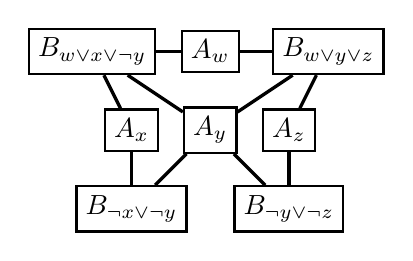
\begin{tikzpicture}
\begin{scope}[every node/.style={thick,draw}]
    \node (C) at (-1,-1) {$B_{\neg x \lor \neg y}$};
    \node (x) at (-1,0) {$A_x$};
    \node (A) at (-1.5,1) {$B_{w \lor x \lor \neg y}$};
    \node (y) at (0,0) {$A_y$};
    \node (w) at (0,1) {$A_w$};
    \node (D) at (1,-1) {$B_{\neg y \lor \neg z}$};
    \node (z) at (1,0) {$A_z$};
    \node (B) at (1.5,1) {$B_{w \lor y \lor z}$};
\end{scope}

\begin{scope}[every node/.style={fill=white,circle},
              every edge/.style={draw=black,very thick}]
    \path [-] (A) edge (w);
    \path [-] (A) edge (x);
    \path [-] (A) edge (y);
    \path [-] (B) edge (w);
    \path [-] (B) edge (y);
    \path [-] (B) edge (z);
    \path [-] (C) edge (x);
    \path [-] (C) edge (y);
    \path [-] (D) edge (y);
    \path [-] (D) edge (z);
\end{scope}
\end{tikzpicture}
	\caption{\label{fig:wmc-example} The tensor network produced by Theorem \ref{thm:wmc-reduction} on $\varphi = (w \lor x \lor \neg y) \land (w \lor y \lor z) \land (\neg x \lor \neg y) \land (\neg y \lor \neg z)$ has 8 tensors (indicated by vertices) and 10 indices (indicated by edges). The $A_*$ tensors correspond to variables and have entries computed from the weight function.  The $B_*$ tensors correspond to clauses and have entries computed from the clause negations.}
\end{figure}
\begin{theorem}
\label{thm:wmc-reduction}
Let $\varphi$ be a CNF formula over Boolean variables $X$ and let $W$ be a weight function. One can construct in polynomial time a tensor network $N_{\varphi,W}$ such that $\tnfree{N_{\varphi,W}} = \emptyset$ and the contraction of $N_{\varphi,W}$ is $W(\varphi)$.
\end{theorem}
\begin{proof}[Sketch of Construction] Let $I = \{(x, C) \in X \times \varphi: x~\text{appears in}~C\}$ be a set of indices, each with domain $\{0,1\}$. The key idea is create a tensor $A_x$ for each variable $x \in X$ and a tensor $B_C$ for each clause $C \in \varphi$ so that each index $(x, C) \in I$ is an index of $A_x$ and $B_C$.

For each $x \in X$, let $A_x$ be a tensor with indices $I \cap (\{x\} \times \varphi)$. For each $\tau \in \domain{I \cap (\{x\} \times \varphi)}$, define $A_x(\tau)$ to be $W(x,0)$ if $\tau$ is always 0, $W(x, 1)$ if $\tau$ is always 1, and 0 otherwise.

For each $C \in \varphi$, let $B_C$ be a tensor with indices $I \cap (X \times \{C\})$. For each $\tau \in \domain{I \cap (X \times \{C\})}$, define $B_C(\tau)$ to be $1$ if $\{x \in X : x~\text{appears in}~C~\text{and}~\tau((x, C)) = 1\}$ satisfies $C$ and 0 otherwise. 

%\begin{multicols}{2}
%    $$A_x(\tau) \equiv \begin{cases}W(x, 0)&\text{if}~\tau~\text{is always 0}\\W(x, 1)&\text{if}~\tau~\text{is always 1}\\0&\text{otherwise.}\end{cases}$$
%  \break
%    $$B_C(\tau) \equiv \begin{cases}1&\text{if}~\{x \in X : x~\text{appears in}~C~\text{and}~\tau((x, C)) = 1\}~\text{satisfies}~C\\0&\text{otherwise.}\end{cases}$$
%\end{multicols}

%For each $x \in X$, define $A_x: [I \cap (\{x\} \times \varphi)] \rightarrow \mathbb{R}$ to be the tensor where $A_x(\tau)$ is $W(x,0)$ if $\tau$ is always 0, $W(x, 1)$ if $\tau$ is always 1, and 0 otherwise. For each $C \in \varphi$, define $B_C: [I \cap (X \times \{C\})] \rightarrow \mathbb{R}$ to be the tensor where $B_C(\tau)$ is $1$ if $\{x \in X : x~\text{appears in}~C~\text{and}~\tau((x, C)) = 1\}$ satisfies $C$ and 0 otherwise. 

Then $N_{\varphi,W} = \{A_x : x \in X\} \cup \{B_C : C \in \varphi\}$ is the desired tensor network.
%Include in $N_{\varphi,W}$ a tensor for each variable and for each clause of $\varphi$. Each variable tensor and clause tensor share an index if and only if the corresponding variable appears in the corresponding clause.
\end{proof}

Theorem \ref{thm:wmc-reduction} proves that $\Call{Reduce}{\varphi,W} = N_{\varphi, W}$ satisfies assumption 1 in Theorem \ref{thm:alg-correctness}. See Figure \ref{fig:wmc-example} for an example of the reduction. This reduction is closely related to the formulation of model counting as the marginalization of a factor graph representing the constraints (but assigns tensors to variables as well, not just clauses). %Unlike the reduction to factor-graph marginalization, which only assigns factors to clauses, Theorem \ref{thm:wmc-reduction} also assigns a tensor to each variable $x$. % For example, if $x$ has weights $W(x, 0) = W(x,1) = 1$ then the tensor assigned to $x$ is a copy tensor. 
This reduction can also be extended to other types of constraints, e.g. parity or cardinality constraints.

\subsection{The Execution Stage}
For formulas $\varphi$ with hundreds of clauses, the corresponding tensor network produced by Theorem \ref{thm:wmc-reduction} has hundreds of bond indices. Directly following Equation \ref{eqn:contraction} in this case is infeasible, since it sums over an exponential number of terms. 

Instead, Algorithm \ref{alg:network-contraction} shows how to compute $\tntensor{N}$ for a tensor network $N$ using a contraction tree $T$ as a guide. The key idea is to repeatedly choose two tensors $A_1, A_2 \in N$ (according to the structure of $T$) and contract them. One can prove inductively that Algorithm \ref{alg:network-contraction} satisfies assumption 3 of Theorem \ref{thm:alg-correctness}.

% Since $N'$ is a partial contraction of $N$, $\tntensor{N'} = \tntensor{N}$. Thus, when this process produces a tensor network containing a single tensor, it follows inductively that this tensor is $\tntensor{N}$. Therefore Algorithm \ref{alg:network-contraction} satisfies assumption 3 of Theorem \ref{thm:alg-correctness}.

\label{sec:algorithm:execution}
\begin{algorithm}[t]
	\caption{Recursively contracting a tensor network}\label{alg:network-contraction}
	\textbf{Input:} A tensor network $N$ and a contraction tree $T$ for $N$. \\
	\textbf{Output:} $\tntensor{N}$, the contraction of $N$.
	\begin{algorithmic}[1]
	    \Procedure{Execute}{$N,T$}
		\If {$\left|N\right| = 1$}
		\State \Return the tensor contained in $N$
		\Else
        \State $T_1, T_2 \gets \text{immediate subtrees of}~T$
		\State \Return $\Call{Execute}{\Lv{T_1}, T_1} \cdot \Call{Execute}{\Lv{T_2}, T_2}$
		\EndIf
		\EndProcedure
	\end{algorithmic}
\end{algorithm}

Each contraction in Algorithm \ref{alg:network-contraction} contains exactly two tensors and so can be implemented as a matrix multiplication. In \cite{DDV19}, \tool{numpy} \cite{numpy} was used to perform each of these contractions. %, but such contractions can also be done with \tool{TensorFlow} \cite{ABCCDDDGII16} and other tensor libraries.
Although the choice of contraction tree does not affect the correctness of Algorithm \ref{alg:network-contraction}, it may have a dramatic impact on the running-time and memory usage. We explore this further in the following section.

\subsection{The Planning Stage}
\label{sec:algorithm:planning}
The task in the planning stage is, given a tensor network, to find a contraction tree that minimizes the computational cost of Algorithm \ref{alg:network-contraction}.

Several \emph{cost-based} approaches \cite{Hirata03,PHV14} aim for minimizing the total number of floating point operations to perform Algorithm \ref{alg:network-contraction}. Most cost-based approaches are designed for tensor networks with very few, large tensors, whereas weighted model counting benchmarks produce tensor networks with many, small tensors. These approaches are thus inappropriate for counting.

Instead, we focus here on \emph{structure-based} approaches, which analyze the rank of intermediate tensors that appear during Algorithm \ref{alg:network-contraction}. The ranks indicate the amount of memory and computation required at each recursive stage. The goal is then to find a contraction tree with small \emph{max-rank}, which is the maximum rank of all tensors that appear during Algorithm \ref{alg:network-contraction}.

This is done through analysis of the \emph{structure graph}, a representation of a tensor network as a graph where tensors are vertices and indices indicate the edges between tensors~\cite{DDV19,MS08,Ying17}:
\begin{definition}[Structure Graph]\label{def:structure}
	Let $N$ be a tensor network. The \emph{structure graph} of $N$ is the graph, denoted $G = \struct{N}$, where $\V{G} = N \cup \{\fv\}$ ($\fv$ is a fresh vertex called the \emph{free vertex}), $\E{G} = \tnbound{N} \cup \tnfree{N}$, $\vinc{G}{\fv} = \tnfree{N}$, and, for all $A \in N$, $\vinc{G}{A} = \tdim{A}$.
	
	%\begin{enumerate}
	%    \item $\V{G} = N \cup \{\fv\}$, where $\fv$ is a fresh vertex called the \emph{free vertex},
	%    \item $\E{G} = \tnbound{N} \cup \tnfree{N}$,
	%    \item each tensor is incident to its indices, and
	%    \item $\fv$ is incident to all free indices.
	%\end{enumerate}
    % That is, $\V{G} = N \sqcup \{ \fv \}$, $\E{G} = \tnbound{N} \cup \tnfree{N}$, $\vinc{G}{A} = \tdim{A}$ for all $A \in N$, and $\vinc{G}{\fv} = \tnfree{N}$.
\end{definition}

%Kourtis et. al \cite{KCMR18} introduced three algorithms for heuristically minimizing the max rank using the structure graph: a greedy algorithm, an algorithm using graph partitioning, and an algorithm using community-structure detection. Another algorithm \cite{MS08,DFGHSW18} utilizes low-width tree decompositions of the line graph of $\struct{N}$. 
%On factor graphs, this approach is analogous to the use of tree decompositions of the primal graph to find variable elimination orders \cite{KDLD05}.

For example, if $\varphi$ is a formula and $N_{\varphi,W}$ is the tensor network resulting from Theorem \ref{thm:wmc-reduction}, then $\struct{N_{\varphi,W}}$ is the incidence graph of $\varphi$ (and is independent of the weight function).

One structure-based approach for finding contraction trees \cite{DFGHSW18,MS08} utilizes low-width tree decompositions of the line graph of $\struct{N}$. This approach is analogous to \emph{variable elimination} on factor graphs \cite{BDP09,KDLD05}, which uses tree decompositions of the primal graph of a factor graph.

Unfortunately, for many tensor network all possible contraction trees have large max-rank. \cite{DDV19} observed that this is the case for many standard counting benchmarks. This is because, for each variable $x$, the number of times $x$ appears in $\varphi$ is a lower bound on the max-rank of all contraction trees of $\Call{Reduce}{\varphi, \cdot}$. Thus traditional tensor network planning algorithms (e.g., \cite{DFGHSW18,KCMR18,MS08}) fail on counting benchmarks that have variables which appear more than $30$ times. 

%For example, if a tensor network contains a rank $k$ tensor, then all contraction trees necessarily have max-rank at least $k$. Recall from Theorem \ref{thm:wmc-reduction} that, for weighted model counting, a variable $x$ that appears $k$ times in $\varphi$ is represented in $\Call{Reduce}{\varphi, W}$ by a rank $k$ tensor. Thus for many weighted model counting benchmarks, where a single variable might appear tens or even hundreds of times, the resulting tensor network will have tensors of infeasibly-high rank. Indeed, 
Instead, \cite{DDV19} relaxed the planning stage by allowing changes to the input tensor network $N$. In particular, \cite{DDV19} used tree decompositions of $\struct{N}$ to factor high-rank, highly-structured tensors as a preprocessing step, following prior methods that split large CNF clauses \cite{SS10_2} and high-degree graph vertices \cite{oliveira18,MS11}. A tensor is highly-structured here if it is \emph{tree-factorable}:
\begin{definition} \label{def:tree-factorable}
A tensor $A$ is \emph{tree factorable} if, for every tree $T$ whose leaves are $\tdim{A}$, there is a tensor network $N_A$ and a bijection $g_A: \V{T} \rightarrow N_A$ s.t. $A$ is the contraction of $N_A$ and:
\begin{enumerate}\itemsep0em 
%\item $A$ is the contraction of $N_A$,
\item $g_A$ is an isomorphism between $T$ and $\struct{N_A}$ with the free vertex removed,
\item for every index $i$ of $A$, $i$ is an index of $g_A(i)$, and
\item for some index $i$ of $A$, every index $j \in \tnbound{N_A}$ satisfies $|\domain{j}| \leq |\domain{i}|$. % the bond dimension of $N_A$ is no bigger than $|\domain{i}|$. % $\max_{i \in \tnbound{N}} |\domain{i}| \leq \max_{i \in \tdim{A}} |\domain{i}|$.
\end{enumerate}
\end{definition}
Informally, a tensor is tree-factorable if it can be replaced by arbitrary trees of low-rank tensors. All tensors produced by Theorem \ref{thm:wmc-reduction} are tree factorable. 
The preprocessing method of \cite{DDV19} is then formalized as follows:
\begin{theorem} \label{thm:factorable-tree}
Let $N$ be a tensor network of tree-factorable tensors such that $|\tnfree{N}| \leq 3$ and $\struct{N}$ has a tree decomposition of width $w \geq 1$. Then we can construct in polynomial time a tensor network $M$ and a contraction tree $T$ for $M$ s.t. $\text{max-rank}(T) \leq \ceil{4(w+1)/3}$ and $N$ is a partial contraction of $M$.
\end{theorem}

This gives us the $\Call{FactorTree}{N}$ planning method, which computes a tree decomposition of $\struct{N}$ and returns the $M$ and $T$ that result from Theorem \ref{thm:factorable-tree}. Because $N$ is a partial contraction of $M$, $\tntensor{N} = \tntensor{M}$. Since all tensors produced by Thereom \ref{thm:wmc-reduction} are tree-factorable, $\Call{FactorTree}{N}$ satisfies assumption 2 in Theorem \ref{thm:alg-correctness}. 

While both $\Call{FactorTree}{N}$ and variable elimination \cite{BDP09,KDLD05} use tree decompositions, they consider different graphs. For example, consider computing the model count of $\psi = \left(\lor_{i=1}^n x_i\right) \land \left(\lor_{i=1}^n \neg x_i\right)$. $\Call{FactorTree}{N}$ uses tree decompositions of the incidence graph of $\psi$, which has treewidth 2. Variable elimination uses tree decompositions of the primal graph of $\psi$, which has treewidth $n-1$. Thus $\Call{FactorTree}{N}$ can exhibit significantly better behavior than variable elimination on some formulas. On the other hand, the behavior of $\Call{FactorTree}{N}$ is at most slightly worse than variable elimination: as noted above, if the treewidth of the primal graph of a formula $\varphi$ is $k$, the treewidth of the incidence graph of $\varphi$ is at most $k+1$ \cite{KV00}. % In the next section we show how branch decompositions can be used to generalize Theorem \ref{thm:factorable-tree} and hence construct contraction trees.